\documentclass[12pt]{article}

\usepackage[OT1]{fontenc} 
\usepackage{amsfonts}
%
%Margin - 1 inch on all sides
%
\usepackage[letterpaper]{geometry}
\usepackage{times}
\geometry{top=1.0in, bottom=1.0in, left=1.0in, right=1.0in}

%
%Doublespacing
%
\usepackage{setspace}
\doublespacing

\usepackage[utf8]{inputenc}
\usepackage{indentfirst}
%
%Rotating tables (e.g. sideways when too long)
%
\usepackage{rotating}

% reference
% !BIB TS-program = biber
% !BIB program = biber
\usepackage[style=numeric, sorting=none]{biblatex}
\addbibresource{src/ref.bib}

%
%Fancy-header package to modify header/page numbering (insert last name)
%
\usepackage{fancyhdr}
\pagestyle{fancy}
\lhead{} 
\chead{} 
\rhead{He \thepage} 
\lfoot{} 
\cfoot{} 
\rfoot{} 
\renewcommand{\headrulewidth}{0pt} 
\renewcommand{\footrulewidth}{0pt} 
%To make sure we actually have header 0.5in away from top edge
%12pt is one-sixth of an inch. Subtract this from 0.5in to get headsep value
\setlength\headsep{0.333in}

%%%%Title
%Begin document
%
\begin{document}

\begin{flushleft}


{\Large\bf Image Generation Models and Their Impact on Japanese Anime Industry} \\
%%%%First page name, class, etc
Ethan He \\

\setlength{\parindent}{0.5in}
%%%%Begin body of paper here
\subsection*{Abstract}
The recent development of deep learning generative models has provided many new insights into drawing and animation.
With the rapid growth of big data and image resources, computer scientists are able to train artificial intelligence (AI) models to generate anime characters or landscape ``paintings.'' 
Considering the tremendous net worth of the Japanese anime industry and related products, drawing and animation have become one of the most important supports of the economy.
When AI was introduced as an ``artist'' and won fine arts competition, the opinions from the animation industry started to diverge.
In this paper, I compare some of the most popular models for the art generation, focusing on the anime drawing generation.
In addition, I analyze the impact of AI artists on the Japanese animation industry along with the opinion of the public and from the related fields of drawing and arts.


\subsection*{Introduction}
\par
Computer vision and image processing are one of the most popular fields of computer science. 
Scientists interpret images as matrices, as images are displaced as a rectangular formation of pixels on our screen.
Academia and industry have made multiple attempts to generate high-quality images
\cite{
    pmlr-v37-gregor15, 
    Qiao_2019_CVPR, 
    NEURIPS2019_1d72310e, 
    NIPS2016_b1301141,
    Goodfellow2020Generative,
    Rombach2022High,
    He_2022_CVPR,
}.
The task of image generation also varies,
but the most studied directions are 
random noise to image,
the text description to the image,
and incomplete image to completed image.
Among these models, Generative Adversarial Networks (GAN) \cite{Goodfellow2020Generative} and Latent Diffusion Models (LDM) \cite{Rombach2022High} are more commonly used for images that are related to art, for example, photography and drawing.

\par
The wave of generative AI is not limited to computer science related academia and industry. 
Jason Allen's artifact created with Midjourney\cite{Midjourney} won first place at the Colorado State Fair's fine arts competition in September 2022 \cite{Teoh2022Art}.
The editor Teoh \cites{Teoh2022Art} further reported that 
``Although the two judges were unaware that Allen's submission was AI-generated, they added that it wouldn't change their decision because they were looking for `how the art tells a story and how it invokes spirit' instead.''
This clearly indicates that the text-to-image generation is capable for storytelling and spirit invoking based on the inputted text description.

\par
Aoi also stated that generative models are about capturing human feelings toward the objects from the text input \cite{Aoi2022Stable}.
Aoi illustrate that both Midjourney and Diffusion model can understand
{\it kawaii} (cute).
{\it Kawaii} is the signature of broadening Japanese culture to the global,
which was created at the time Japanese domestic focus shifted from production to consumption \cite{Yano2013Pink}.
Based on that idea,
% ! use of I
I argue that text-to-image models also have the power to generate anime girl characters,
which is one of the most reflective genres of the Japanese idea of {\it kawaii}.
In fact, there are examples of a customized version of both GAN and Diffusion for anime character generation
\cite{
    Jin2017Towards,
    Ruan2022Anime,
    WaifuDiffusion,
    nizan2020council,
    chong2021gans,
    chong2021jojogan,
}.
\subsection*{Background}

\subsubsection*{GAN}

Generative Adversarial Networks trains a generator $G$ and a discriminator $D$ together though a mini-max game
The generator takes in random noise and maps the noise to an image.
The discriminator takes in an image and tells if it is real from the dataset or generated by the generator.
To train these two network simultaneously, Goodfellow et al. defined the loss function as 
$$
\min_G\max_{D}\mathcal{L}(D, G) = 
\mathbb{E}_{x \sim p_{data}}[\log D(x)] + 
\mathbb{E}_{z \sim p_z}[\log (1 - D(G(z)))]
$$
where $p_{data}$ is the images in the real dataset
and $p_z$ is randomly generated vectors in the same shape as the real images \cite{Goodfellow2020Generative}.

\par
Based on the above models, Karras et al. proposed StyleGAN as 
a GAN variant that can separate high-level feature variations and scale-specific control these variations \cite{Karras2019Style}.
If trained on a dataset of human faces, these high-level features including eyes, nose, hair, etc.
Together with GAN's two model nature, mapping the high-level features of anime characters to real human pictures becomes possible.
Min Jin Chong and Davis Forsyth proposed two GAN-based models,
GANs N' Roses (GNR) and JoJoGAN,
to map anime image style to human pictures \cite{chong2021gans,chong2021jojogan}.
GNR trained on different anime characters will learn different styles,
thus produces a sequence of diverse outputs based on the same input image.
\begin{figure}[h]
    \includegraphics[width=\textwidth]{img/GNR-1.png}
    \caption{
        GANs N' Roses: The first column on the left is the input human picture.
        Each following column shows a different style learned from different anime mapped to that human \cite{chong2021gans}.
    }
\end{figure}

JoJoGAN, however, takes in an anime character's image as reference and generates
a style mapper that can be applied to human faces.
The key difference between JoJoGAN and GNR is that GNR needs a dataset of same anime character to learn the style of that character.
Instead of finding a large amount of quality images of same character,
JoJoGAN can be trained on a generalized anime dataset,
then produce the need style map based on the given single reference.
This difference allows JoJoGAN to generate multiple images of multiple much easier than other style-based image generator.
\begin{figure}[h]
    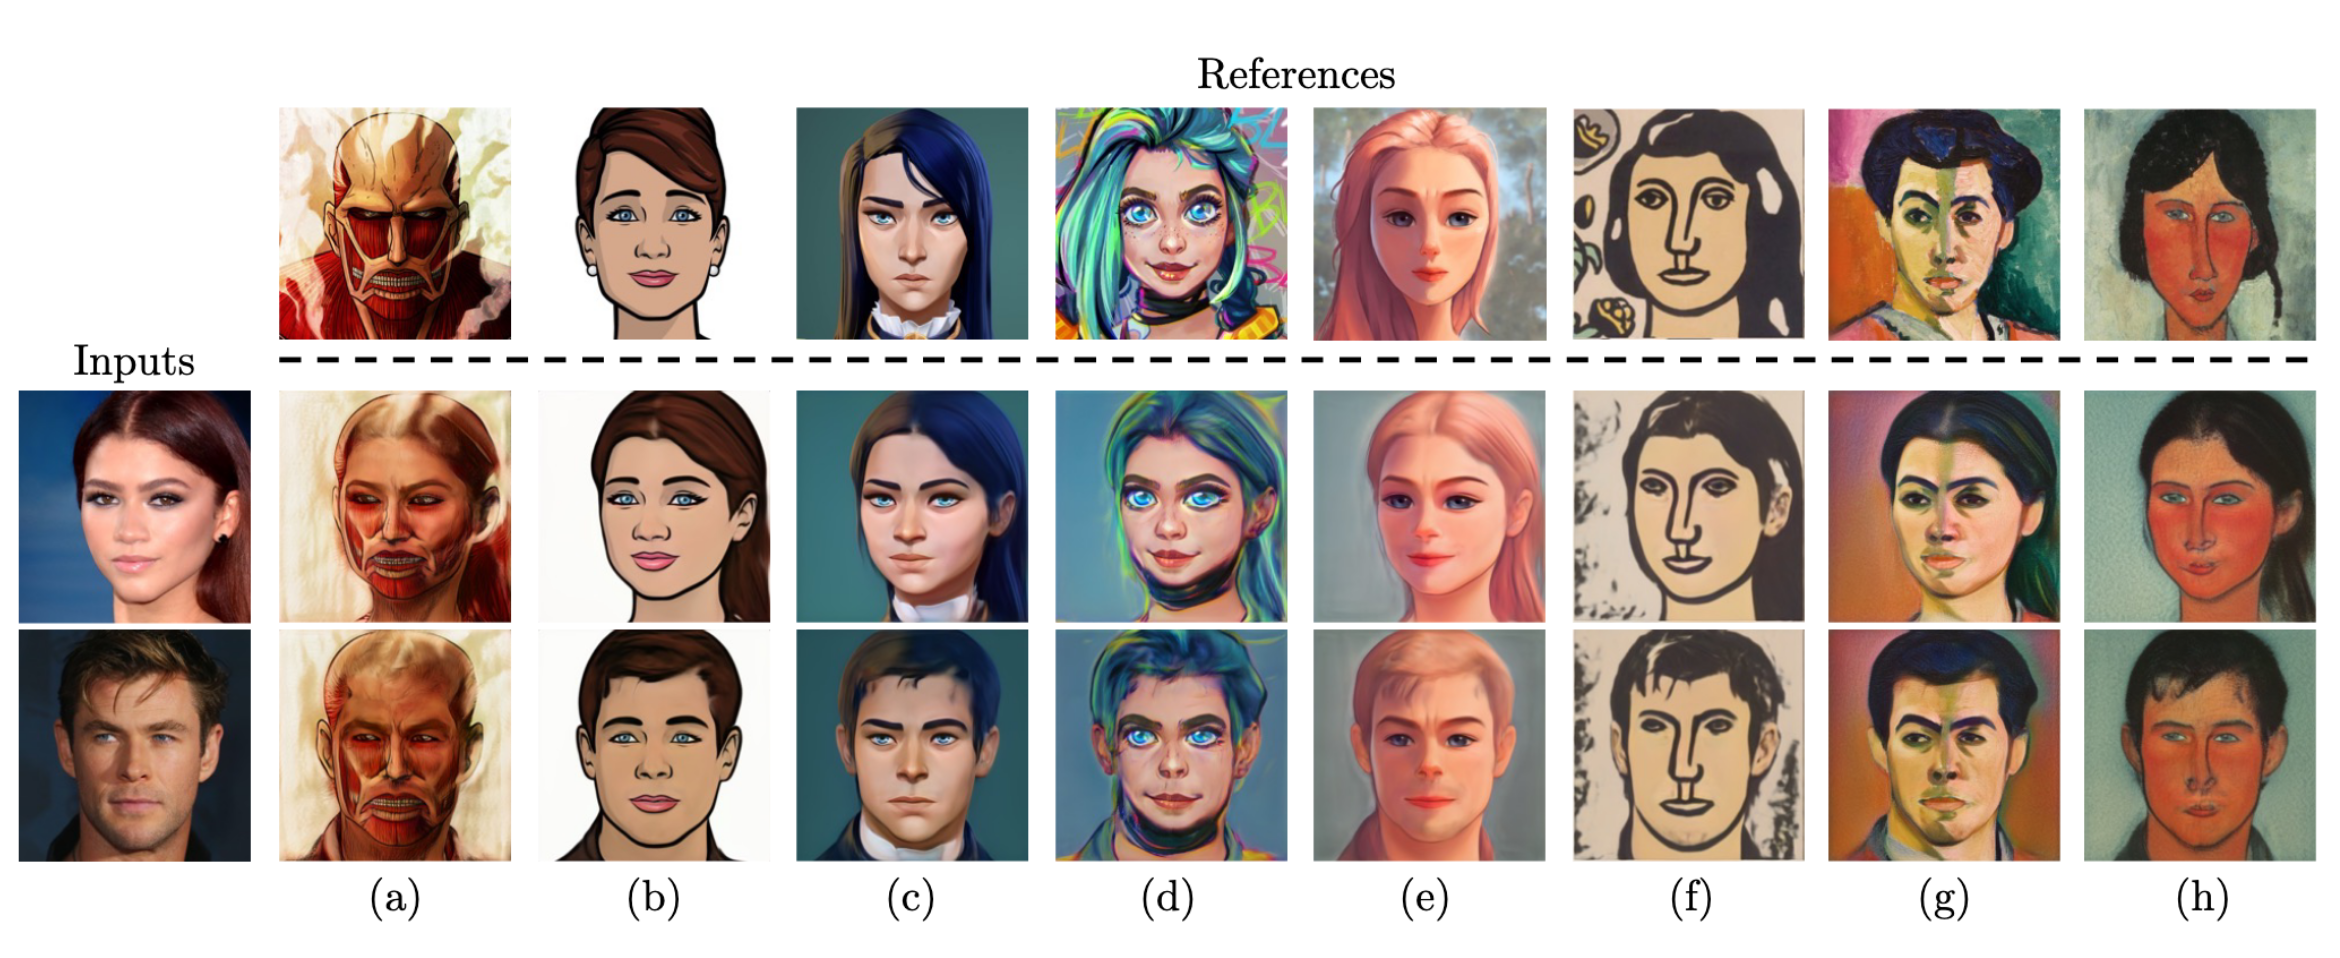
\includegraphics[width=\textwidth]{img/JoJo-1.png}
    \caption{
        JoJoGAN: The first column on the left is the input human picture.
        Each following column shows a different style generated from different reference anime image \cite{chong2021jojogan}.
    }
\end{figure}

\subsubsection*{Diffusion Models}

Rombach et al. newly proposed Latent Diffusion Models as the state-of-art image generation algorithm \cite{Rombach2022High}.
The idea of diffusion is to learn an image style by denoising the training image to learn the data distribution in the image.
That is, gradually break down am image into noises.
Then for generation, they use the inverse map of diffusion to resample on noise under known distribution

$$
L_{L D M}:=\mathbb{E}_{\mathcal{E}(x), \epsilon \sim \mathcal{N}(0,1), t}\left[\left\|\epsilon-\epsilon_\theta\left(z_t, t\right)\right\|_2^2\right]
$$

As StyleGAN models specialized on image-to-image generation,
LDMs shows surprising results on text-to-image generation as shown in Figure 3.
\begin{figure}[]
    \includegraphics[width=\textwidth]{img/LDM-1.png}
    \caption{
        Latent Diffusion Models:
        user input text are on the top
        and the generated images are under the text descriptions \cite{Rombach2022High}.
    }
\end{figure}

When we apply LDM to anime characters,
we can easily generate any character as we want with proper text description as in Figure 4.
As shown in the image grid,
text-to-image generated images are like brand-new characters,
i.e. there is hard to find the exact same style character in existing anime as in StyleGAN generated images.
\begin{figure}[h]
    \begin{center}
    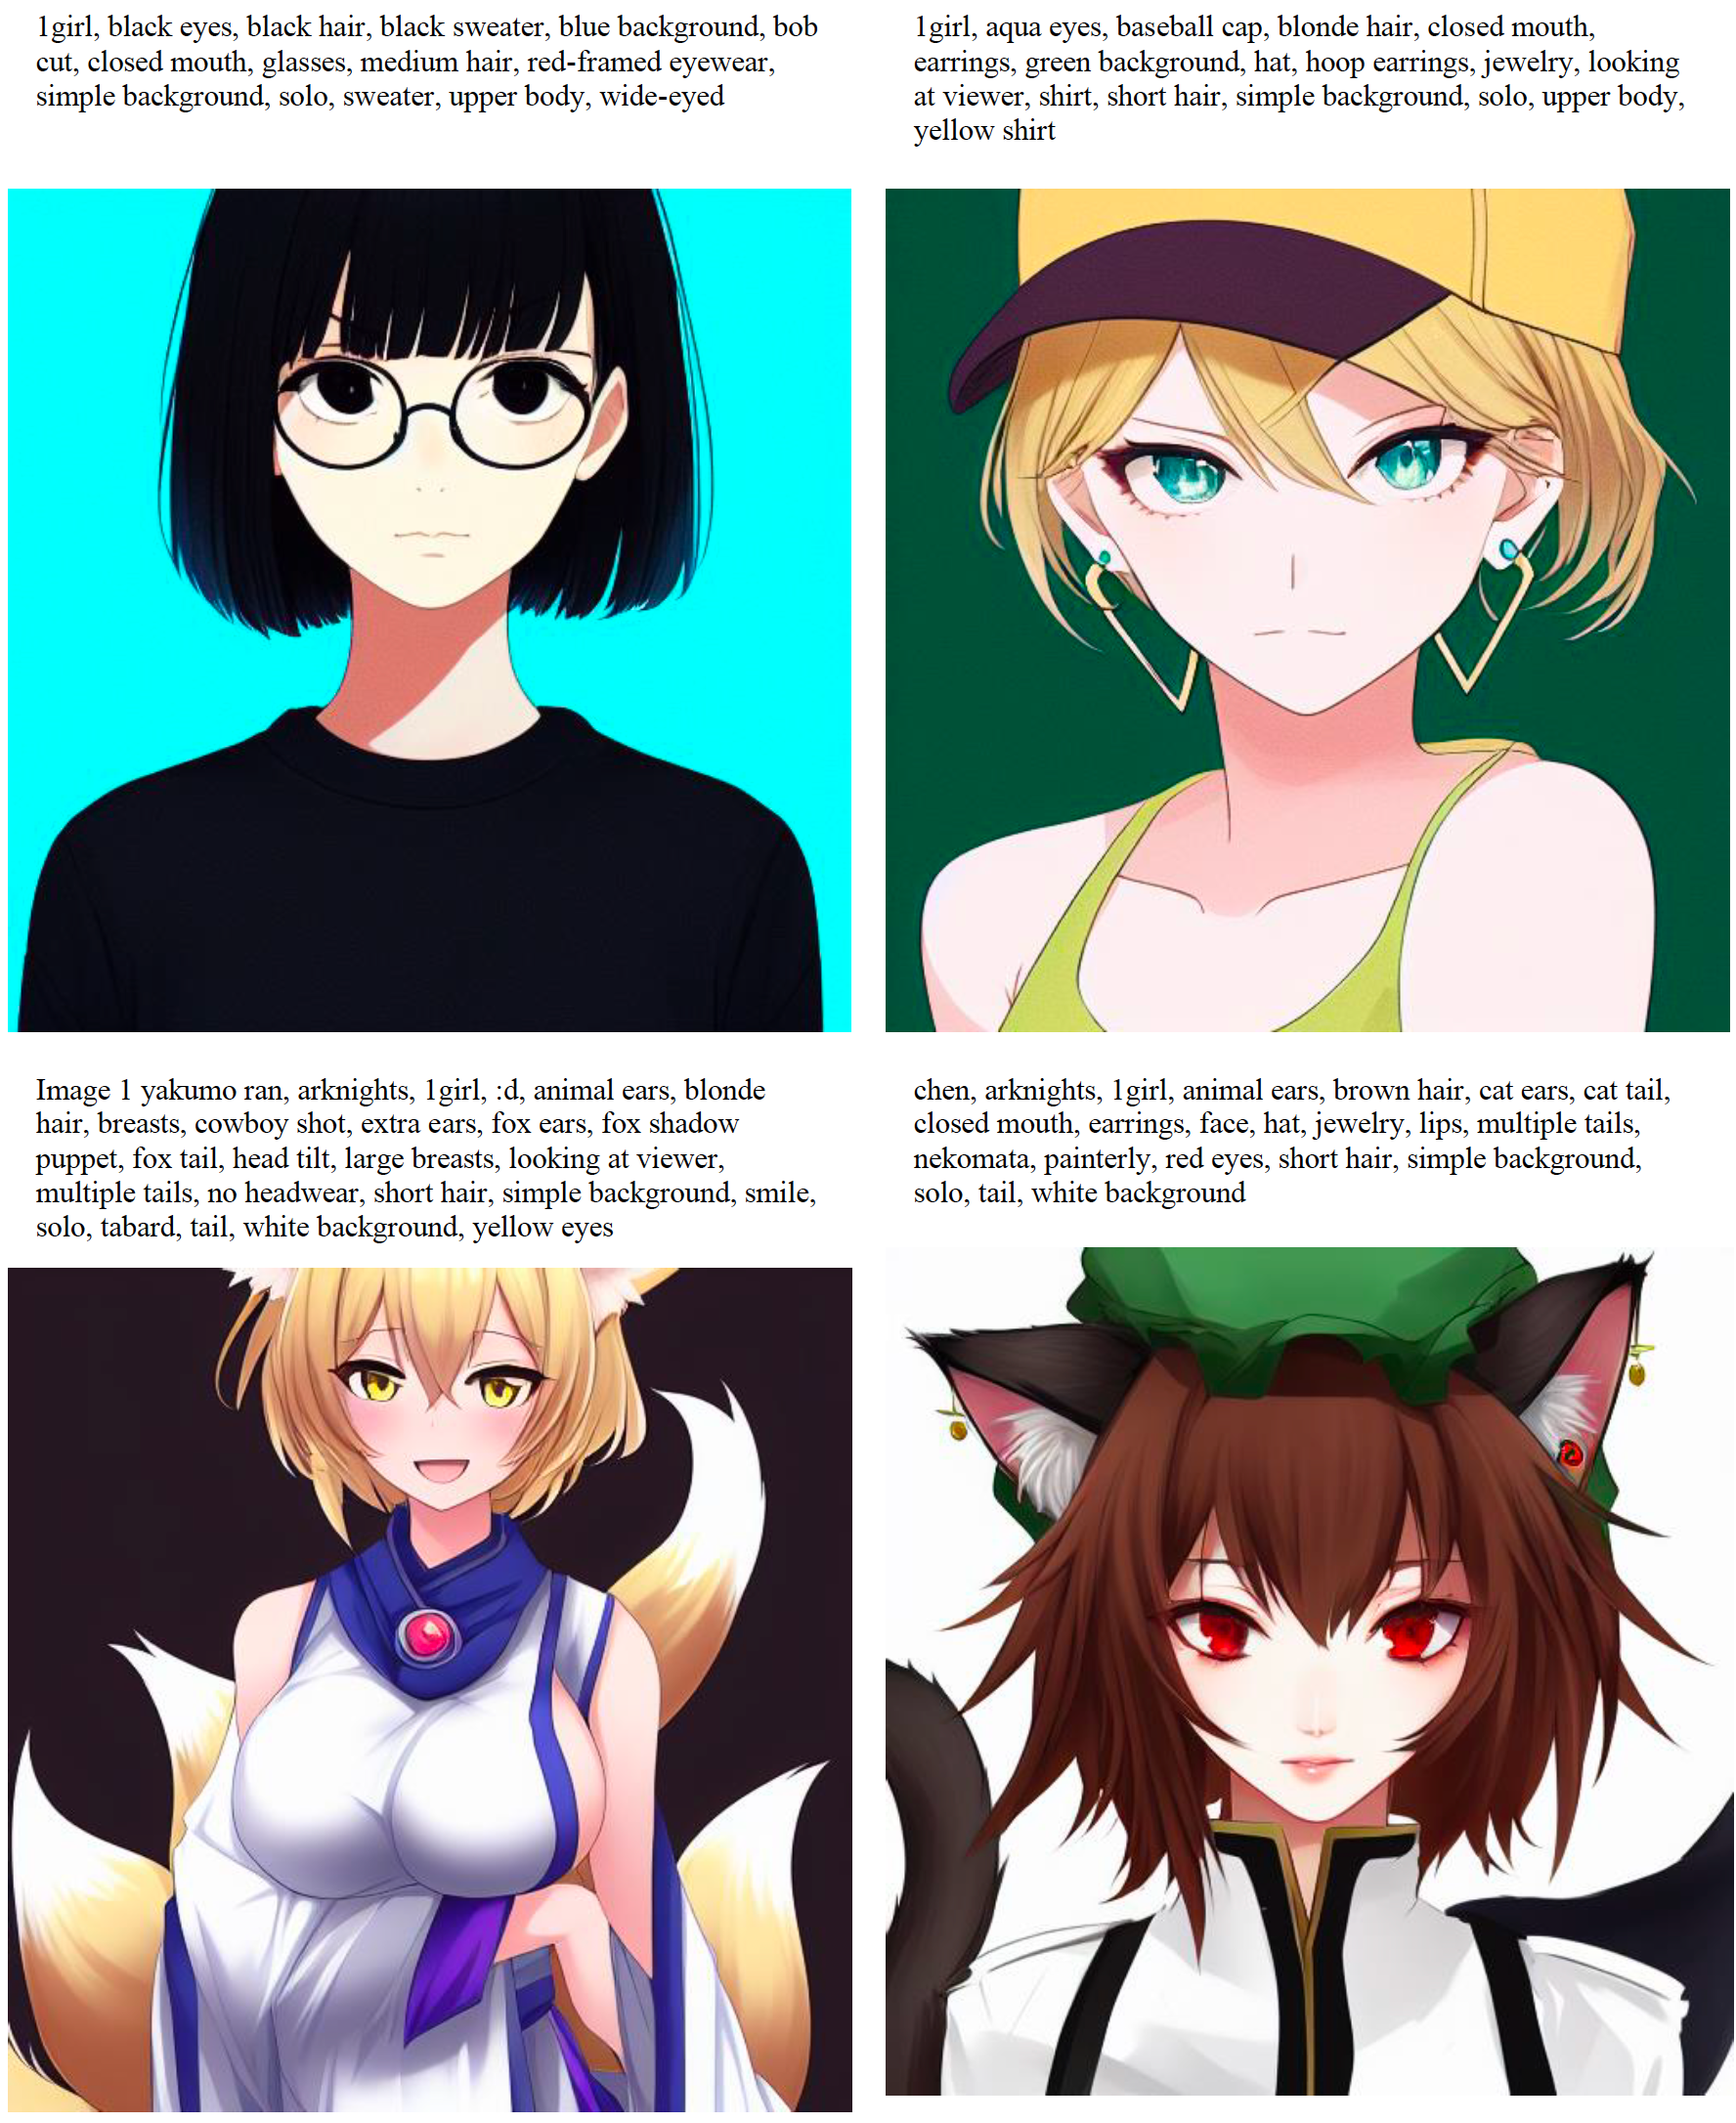
\includegraphics[width=0.78\textwidth]{img/waifu_diffusion.png}
    \end{center}
    \caption{
        Waifu Diffusion:
        user input text are on the top
        and the generated images are under the text descriptions \cite{WaifuDiffusion}.
    }
\end{figure}
\section*{Reaction of Japanese Anime Industry}
\section*{Conclusion}

\newpage
\printbibliography[heading=subbibliography]

\end{flushleft}
\end{document}